% !TEX root = main.tex

\section{Introduction}

Understanding the factors that predict crime is important because even though crime rates have been generally declining since the early nineties, recent years have started to see lower rates of decline and even some upward fluctuations after 2010~\cite{BJS16}. Moreover, reports of direct and indirect victimization and exposures to crime remain very high~\cite{TjLl15}. For instance, more than two-fifths of children and youth in a recent national survey reported a physical assault in the previous year~\cite{FTSH13}.  Understanding the neighborhood context of crime is particularly important because victimization and other forms of crime exposures have many severe consequences.  Beyond the high medical bills and violent death, consequences include behavioral and mental health problems, aggression, substance abuse, post-traumatic stress disorder, and suicide, lower academic achievement, and engaging in further violence~\cite{Grai15}.

In this paper, we study the problem of crime rate inference across communities. We select Chicago as the target of study for the following reason. Chicago has more homicides and non-negligent manslaughter rates (15.2) per 100,000 residents than New York (4.0) and Los Angeles (6.5) according to the FBI crime statistics for 2013 and has experienced no decline in the past decade compared to the other two large cities, which have been on a slow declining slope \cite{crime-stats}.


Traditionally, researchers have used demographic information based on Decennial Census (e.g., population poverty level, socioeconomic disadvantage, racial composition of population) to estimate the crime rate in a community~\cite{GrSa09}. However,  such information only contains the social information of residents in the neighborhoods and misses information on daily population dynamics within and between neighborhoods. In our experiments (Section~\ref{sec:experiment}), negative binomial and geographically weighted negative binomial models that only use demographic features and an intercept result in a relative error of as much as 30\% for crime rate estimation in Chicago. Existing studies also highlight the importance of geographical influence~\cite{Ans02} in estimating crime rates, i.e., the crime in the nearby communities can be propagated to the focal community. But, depending on the geographic scale of analysis, geographical influence does not contribute a great deal in improving the crime inference on top of demographic feature (with at most $0.4\%$ relative improvement in our experiments focused on larger geographic units than census tracts). This is probably because the nearby communities also share similar demographics, which limits the additional benefit of geographical influence.
 
\begin{figure}[t]
\centering
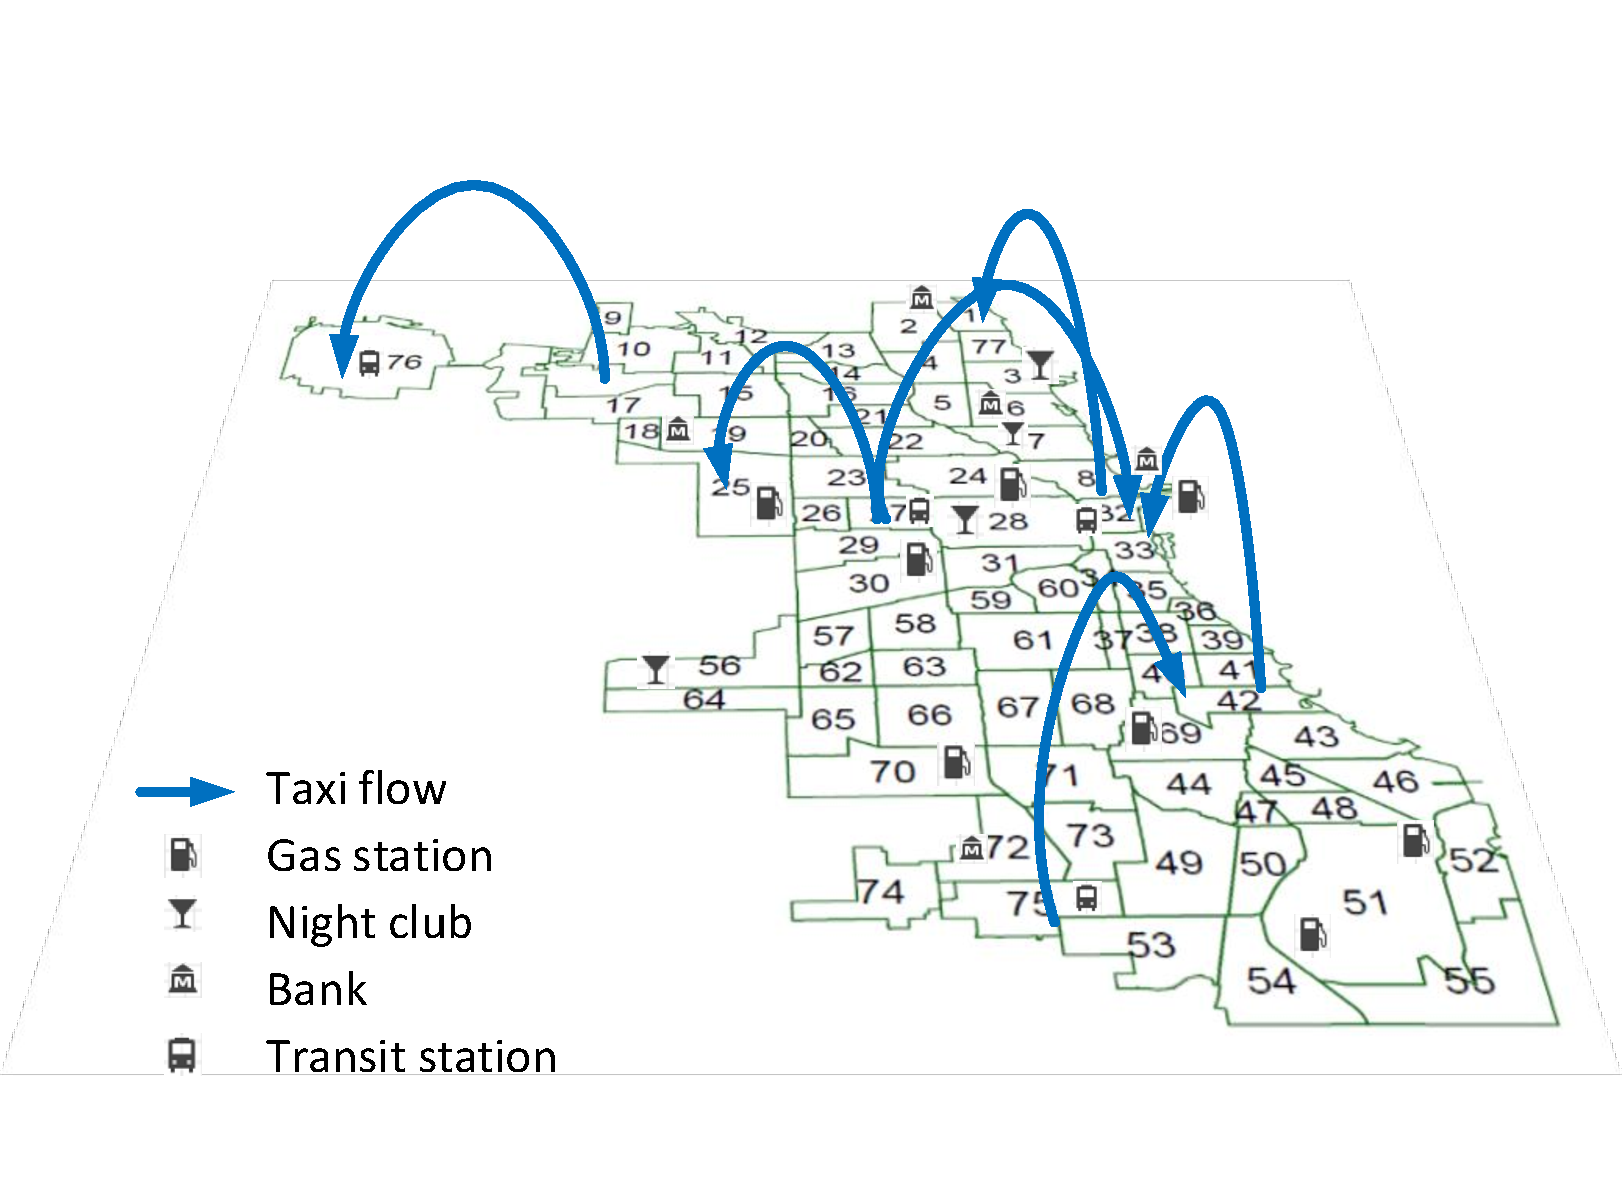
\includegraphics[width=0.8\linewidth]{fig/demo-kdd16.pdf}
\caption{An illustration of various types of features we use in Chicago. The POI distributions across community areas profile the region functionality. The taxi flows connect non-adjacent regions and act as ``hyperlinks'' on the space.}
\label{fig:demo}
\vspace{-3mm}
\end{figure}

Recently, big data reflecting city dynamics have become widely available~\cite{ZCWY14}, e.g., traffic flow, human mobility, social media, and crowd-generated Points-Of-Interest (POI). As shown in Figure~\ref{fig:demo}, such newer types of big data could provide new insights to advance our understanding of traditional socioeconomic urban problems, such as the crime rate inference problem we focus on in this paper. In particular, we propose to study two newer types of urban data: POI and taxi flow. 

\textbf{POI data.} POI data provide venue information such as GPS coordinates, category, popularity, and reviews. These POIs mostly belong to categories such as food, shop, transit, education, etc. As one example, the POI data reveal locations of gas stations and convenience stores, which are more likely to be targets for crime because of lack of guardianship, easy to access, and presence of readily attainable valuables~\cite{EJWD15}. Recent studies have also shown that using such categorical information of POIs are helpful to profile neighborhood functions~\cite{YZX12}. Such neighborhood functions could further help us predict crime rate (e.g., communities with less education or entertainment facilities may have a higher rate of crime). 
%Our experiments show that incorporating POI features significantly improve the crime rate inference. Adding POI features in addition to demographics features reduces the relative error by at least $5\%$ in our experiments. This demonstrates that POI data provide additional information about the communities that is not covered by the demographics.

\textbf{Taxi flow data.} A huge amount of taxi flow data reflect important information about how people move across neighborhoods in the city. In previous studies, when using geographical influence~\cite{Ans02}, scientists assume that a community is affected by other spatially proximate communities. However, even if two communities are distant in geographical space, they could be strongly correlated if many people frequently travel between these two communities~\cite{GGM14}. We hypothesize that taxi flows may be considered as ``hyperlinks'' in the city that connect different areas and we use such data to estimate crime rates. 
We do not expect taxi flow data to capture the movements of offenders, as the vast majority of taxi trips are probably unrelated to crime. Instead, we view taxi flow as a proxy for broader patterns of population routine activity and mobility, commuting flows, and other forms of social and economic exchanges between two communities over space. Such exchanges may increase the number of potential targets and opportunities for crime \cite{CLFM79,BPBP95} or contribute to inter-community diffusion of information about successful local strategies to control  or prevent crime (e.g., successful features of neighborhood watch programs). 
%Our experiments show very promising results --  adding taxi flow data on top of all other features can further decrease the error by 5\%.

We apply various regression models to 5 years of crime data in Chicago. The most frequently used model is linear regression; however, because crime count cannot be negative, we also use negative binomial regression.  We demonstrate that negative binomial model generally performs better than the linear regression. In addition, adding POI and taxi flow features reduces the relative error by at least 5\% in our experiments. This indicates that the new urban data provide additional information about the communities which are not covered by traditional features.

As an extension to the conference version~\cite{WKGL16}, we investigate models that incorporate geographic heterogeneity; that is, we do not expect the same features to have the same relation to crime in every location because crime incidents in different regions may be associated with different social-economic factors.
In fact, there are several neighborhoods where negative binomial model gives poor prediction. This tells us that a global model such as the negative binomial model, which assumes a constant correlation between crime and observed features, would not yield accurate estimates. Therefore, we further propose to employ a graphically weighted regression approach to capture the non-stationary property of crime. The intuition behind this strategy is to train many local models instead of one global model to predict the crime. The geographically weighted regression is a useful framework on how to pick samples and weight them for local model training. We thus apply geographically weighted regression in combination with negative binomial model, and the experiments show further improvements over the global model.


In summary, the contributions of this paper are:  1) We study an old but important crime inference problem by utilizing new urban data: POIs and taxi flows. We provide detailed discussions of how to construct features, tests of different combinations of features, and the theoretical interpretations of the result from a social scientist (a co-author in the paper). 2) We find that utilizing these new types of big urban data improves the crime rate inference. 3) We employ a geographically weighted regression framework to capture the non-stationary property of crime. 4) We conduct a systematic comparison between various regression models. The geographically weighted negative binomial model has significantly better performance, and could serve as a new baseline for future crime inference problems.

The rest of this paper is organized as follows. We first review the related work in Section \ref{sec:related-work}. The crime inference problem is formulated in Section \ref{sec:overview}. We discuss the inference model in Section \ref{sec:model} and feature extraction procedure in Section \ref{sec:feature}. The Section \ref{sec:experiment} presents the quantitative evaluation results on real data. Finally, we conclude the paper in Section \ref{sec:conclusion}.

